\documentclass[]{article}
\usepackage{lmodern}
\usepackage{amssymb,amsmath}
\usepackage{ifxetex,ifluatex}
\usepackage{fixltx2e} % provides \textsubscript
\ifnum 0\ifxetex 1\fi\ifluatex 1\fi=0 % if pdftex
  \usepackage[T1]{fontenc}
  \usepackage[utf8]{inputenc}
\else % if luatex or xelatex
  \ifxetex
    \usepackage{mathspec}
  \else
    \usepackage{fontspec}
  \fi
  \defaultfontfeatures{Ligatures=TeX,Scale=MatchLowercase}
\fi
% use upquote if available, for straight quotes in verbatim environments
\IfFileExists{upquote.sty}{\usepackage{upquote}}{}
% use microtype if available
\IfFileExists{microtype.sty}{%
\usepackage{microtype}
\UseMicrotypeSet[protrusion]{basicmath} % disable protrusion for tt fonts
}{}
\usepackage[margin=1in]{geometry}
\usepackage{hyperref}
\hypersetup{unicode=true,
            pdfborder={0 0 0},
            breaklinks=true}
\urlstyle{same}  % don't use monospace font for urls
\usepackage{color}
\usepackage{fancyvrb}
\newcommand{\VerbBar}{|}
\newcommand{\VERB}{\Verb[commandchars=\\\{\}]}
\DefineVerbatimEnvironment{Highlighting}{Verbatim}{commandchars=\\\{\}}
% Add ',fontsize=\small' for more characters per line
\usepackage{framed}
\definecolor{shadecolor}{RGB}{248,248,248}
\newenvironment{Shaded}{\begin{snugshade}}{\end{snugshade}}
\newcommand{\KeywordTok}[1]{\textcolor[rgb]{0.13,0.29,0.53}{\textbf{#1}}}
\newcommand{\DataTypeTok}[1]{\textcolor[rgb]{0.13,0.29,0.53}{#1}}
\newcommand{\DecValTok}[1]{\textcolor[rgb]{0.00,0.00,0.81}{#1}}
\newcommand{\BaseNTok}[1]{\textcolor[rgb]{0.00,0.00,0.81}{#1}}
\newcommand{\FloatTok}[1]{\textcolor[rgb]{0.00,0.00,0.81}{#1}}
\newcommand{\ConstantTok}[1]{\textcolor[rgb]{0.00,0.00,0.00}{#1}}
\newcommand{\CharTok}[1]{\textcolor[rgb]{0.31,0.60,0.02}{#1}}
\newcommand{\SpecialCharTok}[1]{\textcolor[rgb]{0.00,0.00,0.00}{#1}}
\newcommand{\StringTok}[1]{\textcolor[rgb]{0.31,0.60,0.02}{#1}}
\newcommand{\VerbatimStringTok}[1]{\textcolor[rgb]{0.31,0.60,0.02}{#1}}
\newcommand{\SpecialStringTok}[1]{\textcolor[rgb]{0.31,0.60,0.02}{#1}}
\newcommand{\ImportTok}[1]{#1}
\newcommand{\CommentTok}[1]{\textcolor[rgb]{0.56,0.35,0.01}{\textit{#1}}}
\newcommand{\DocumentationTok}[1]{\textcolor[rgb]{0.56,0.35,0.01}{\textbf{\textit{#1}}}}
\newcommand{\AnnotationTok}[1]{\textcolor[rgb]{0.56,0.35,0.01}{\textbf{\textit{#1}}}}
\newcommand{\CommentVarTok}[1]{\textcolor[rgb]{0.56,0.35,0.01}{\textbf{\textit{#1}}}}
\newcommand{\OtherTok}[1]{\textcolor[rgb]{0.56,0.35,0.01}{#1}}
\newcommand{\FunctionTok}[1]{\textcolor[rgb]{0.00,0.00,0.00}{#1}}
\newcommand{\VariableTok}[1]{\textcolor[rgb]{0.00,0.00,0.00}{#1}}
\newcommand{\ControlFlowTok}[1]{\textcolor[rgb]{0.13,0.29,0.53}{\textbf{#1}}}
\newcommand{\OperatorTok}[1]{\textcolor[rgb]{0.81,0.36,0.00}{\textbf{#1}}}
\newcommand{\BuiltInTok}[1]{#1}
\newcommand{\ExtensionTok}[1]{#1}
\newcommand{\PreprocessorTok}[1]{\textcolor[rgb]{0.56,0.35,0.01}{\textit{#1}}}
\newcommand{\AttributeTok}[1]{\textcolor[rgb]{0.77,0.63,0.00}{#1}}
\newcommand{\RegionMarkerTok}[1]{#1}
\newcommand{\InformationTok}[1]{\textcolor[rgb]{0.56,0.35,0.01}{\textbf{\textit{#1}}}}
\newcommand{\WarningTok}[1]{\textcolor[rgb]{0.56,0.35,0.01}{\textbf{\textit{#1}}}}
\newcommand{\AlertTok}[1]{\textcolor[rgb]{0.94,0.16,0.16}{#1}}
\newcommand{\ErrorTok}[1]{\textcolor[rgb]{0.64,0.00,0.00}{\textbf{#1}}}
\newcommand{\NormalTok}[1]{#1}
\usepackage{graphicx,grffile}
\makeatletter
\def\maxwidth{\ifdim\Gin@nat@width>\linewidth\linewidth\else\Gin@nat@width\fi}
\def\maxheight{\ifdim\Gin@nat@height>\textheight\textheight\else\Gin@nat@height\fi}
\makeatother
% Scale images if necessary, so that they will not overflow the page
% margins by default, and it is still possible to overwrite the defaults
% using explicit options in \includegraphics[width, height, ...]{}
\setkeys{Gin}{width=\maxwidth,height=\maxheight,keepaspectratio}
\IfFileExists{parskip.sty}{%
\usepackage{parskip}
}{% else
\setlength{\parindent}{0pt}
\setlength{\parskip}{6pt plus 2pt minus 1pt}
}
\setlength{\emergencystretch}{3em}  % prevent overfull lines
\providecommand{\tightlist}{%
  \setlength{\itemsep}{0pt}\setlength{\parskip}{0pt}}
\setcounter{secnumdepth}{0}
% Redefines (sub)paragraphs to behave more like sections
\ifx\paragraph\undefined\else
\let\oldparagraph\paragraph
\renewcommand{\paragraph}[1]{\oldparagraph{#1}\mbox{}}
\fi
\ifx\subparagraph\undefined\else
\let\oldsubparagraph\subparagraph
\renewcommand{\subparagraph}[1]{\oldsubparagraph{#1}\mbox{}}
\fi

%%% Use protect on footnotes to avoid problems with footnotes in titles
\let\rmarkdownfootnote\footnote%
\def\footnote{\protect\rmarkdownfootnote}

%%% Change title format to be more compact
\usepackage{titling}

% Create subtitle command for use in maketitle
\providecommand{\subtitle}[1]{
  \posttitle{
    \begin{center}\large#1\end{center}
    }
}

\setlength{\droptitle}{-2em}

  \title{}
    \pretitle{\vspace{\droptitle}}
  \posttitle{}
    \author{}
    \preauthor{}\postauthor{}
    \date{}
    \predate{}\postdate{}
  

\begin{document}

\section{Data Analysis in R}\label{data-analysis-in-r}

Adam Rawles

\subsection{Recap}\label{recap}

\begin{itemize}
\tightlist
\item
  What is R and RStudio?
\item
  Basic arithmetic operators
\item
  Variable assigment
\item
  Data types
\item
  Data structures (including subsetting)
\item
  Functions
\end{itemize}

\subsection{Overview}\label{overview}

\begin{itemize}
\tightlist
\item
  Installing packages
\item
  Loading data
\item
  Cleaning data
\item
  Summary statistics
\item
  Graphs and plots
\end{itemize}

\subsection{Installing packages}\label{installing-packages}

\begin{itemize}
\tightlist
\item
  Installing packages with RStudio is easy to do
\item
  RStudio has a built-in interface for installing packages\ldots{}
\item
  Or, you can use the R function ``install.packages()'', and provide the
  name of the package(s) you want to install to the function
\end{itemize}

\begin{Shaded}
\begin{Highlighting}[]
\KeywordTok{install.packages}\NormalTok{(}\StringTok{"ggplot2"}\NormalTok{)}
\KeywordTok{install.packages}\NormalTok{(}\KeywordTok{c}\NormalTok{(}\StringTok{"ggplot2"}\NormalTok{, }\StringTok{"dplyr"}\NormalTok{))}
\end{Highlighting}
\end{Shaded}

\begin{itemize}
\tightlist
\item
  Packages must be loaded before they are available, via the library()
  function
\end{itemize}

\begin{Shaded}
\begin{Highlighting}[]
\KeywordTok{library}\NormalTok{(ggplot2)}
\end{Highlighting}
\end{Shaded}

\begin{itemize}
\tightlist
\item
  Note: if you close RStudio, you'll need to reload your packages
\end{itemize}

\subsection{Loading data}\label{loading-data}

\begin{itemize}
\tightlist
\item
  Data can be loaded into R in many formats
\item
  The easiest of which are .xlsx or .csv files
\item
  These can be loaded into R two different ways

  \begin{itemize}
  \tightlist
  \item
    The first is by using the read.csv()/read.xlsx() functions

    \begin{itemize}
    \tightlist
    \item
      The read.csv() function takes a string of the file's path as it's
      only required input argument

      \begin{itemize}
      \tightlist
      \item
        But there are a number of optional arguments (e.g.~header,
        stringsAsFactor,\ldots{})
      \end{itemize}
    \item
      The read.xlsx() function requires both a path, and the index of
      the sheet you want from the workbook
    \end{itemize}
  \end{itemize}
\end{itemize}

\subsection{Loading data}\label{loading-data-1}

\begin{itemize}
\tightlist
\item
  The second is to use RStudio's built in ``Import Dataset'' interface

  \begin{itemize}
  \tightlist
  \item
    This interface essentially just acts as a wrapper to the
    read.csv()/xlsx() functions
  \end{itemize}
\end{itemize}

\subsection{Loading data - example}\label{loading-data---example}

\subsection{Loading data - example}\label{loading-data---example-1}

\begin{Shaded}
\begin{Highlighting}[]
\NormalTok{consdata <-}\StringTok{ }\KeywordTok{read.csv}\NormalTok{(}\StringTok{"consdata.csv"}\NormalTok{, }\DataTypeTok{header =} \OtherTok{TRUE}\NormalTok{, }\DataTypeTok{stringsAsFactors =} \OtherTok{TRUE}\NormalTok{)}

\KeywordTok{head}\NormalTok{(consdata, }\DataTypeTok{n =} \DecValTok{2}\NormalTok{)}
\end{Highlighting}
\end{Shaded}

\begin{verbatim}
##   settlement_date settlement_period metered_entity_type metered_entity
## 1      01/01/2018                 1                MPAN       testmpan
## 2      01/01/2018                 2                MPAN       testmpan
##   meter_reading actual_estimate avg_temperature_c
## 1        0.8889               E              7.40
## 2        0.8899               E              7.38
\end{verbatim}

\subsection{Loading data - exercise}\label{loading-data---exercise}

\begin{itemize}
\tightlist
\item
  Using RStudio's ``Import Dataset'' or the read.csv() function, load
  the cons\_data dataset
\end{itemize}

\subsection{Data cleaning}\label{data-cleaning}

\begin{itemize}
\tightlist
\item
  After the data is loaded into R, we need to make sure that each column
  is in the correct format (e.g.~character, factor, numeric, etc.)
\item
  This can be done two different ways:

  \begin{itemize}
  \tightlist
  \item
    You can either click on the dataframe in the Environment pane, which
    will open the dataframe in the Source pane

    \begin{itemize}
    \tightlist
    \item
      From here, you can hover over the column headers to see what type
      the data is stored as
    \end{itemize}
  \item
    Or, you can use the is.xxxxx functions to check from the console.

    \begin{itemize}
    \tightlist
    \item
      To do this, you choose the appropriate function for the type you
      want (e.g.~is.numeric()), and include the column you want to check
      as an argument
    \end{itemize}
  \end{itemize}
\end{itemize}

\subsection{Data cleaning}\label{data-cleaning-1}

\begin{Shaded}
\begin{Highlighting}[]
\KeywordTok{is.numeric}\NormalTok{(consdata}\OperatorTok{$}\NormalTok{meter_reading) ## we could also do is.numeric(consdata[,1]) as per our last session on subsetting}
\end{Highlighting}
\end{Shaded}

\begin{verbatim}
## [1] TRUE
\end{verbatim}

\begin{Shaded}
\begin{Highlighting}[]
\KeywordTok{is.numeric}\NormalTok{(consdata}\OperatorTok{$}\NormalTok{actual_estimate)}
\end{Highlighting}
\end{Shaded}

\begin{verbatim}
## [1] FALSE
\end{verbatim}

\begin{Shaded}
\begin{Highlighting}[]
\KeywordTok{is.factor}\NormalTok{(consdata}\OperatorTok{$}\NormalTok{actual_estimate)}
\end{Highlighting}
\end{Shaded}

\begin{verbatim}
## [1] TRUE
\end{verbatim}

\subsection{Data cleaning}\label{data-cleaning-2}

\begin{itemize}
\tightlist
\item
  If you want to get the type of a column without comparing it to other
  types, you use the is() function
\item
  The first value returned from this function will tell you the data
  type of the column
\end{itemize}

\begin{Shaded}
\begin{Highlighting}[]
\KeywordTok{is}\NormalTok{(consdata}\OperatorTok{$}\NormalTok{meter_reading)}
\end{Highlighting}
\end{Shaded}

\begin{verbatim}
## [1] "numeric" "vector"
\end{verbatim}

\begin{Shaded}
\begin{Highlighting}[]
\KeywordTok{is}\NormalTok{(consdata}\OperatorTok{$}\NormalTok{actual_estimate)}
\end{Highlighting}
\end{Shaded}

\begin{verbatim}
## [1] "factor"              "integer"             "oldClass"           
## [4] "numeric"             "vector"              "data.frameRowLabels"
\end{verbatim}

\subsection{Data cleaning}\label{data-cleaning-3}

\begin{itemize}
\tightlist
\item
  If a column does not have the correct type, we can easily coerce the
  values into the type that we want
\item
  The exact method is different depending on what you are converting
  from and to
\item
  Generally speaking however, the method for converting a column type
  is:
\end{itemize}

\begin{Shaded}
\begin{Highlighting}[]
\NormalTok{dataframe}\OperatorTok{$}\NormalTok{column <-}\StringTok{ }\KeywordTok{as.xxxxx}\NormalTok{(dataframe}\OperatorTok{$}\NormalTok{column)}
\end{Highlighting}
\end{Shaded}

\subsection{Data cleaning - exercise}\label{data-cleaning---exercise}

\begin{itemize}
\tightlist
\item
  Convert the meter reading column into a character, check that it's
  been converted, and then convert it back to numeric
\end{itemize}

\begin{Shaded}
\begin{Highlighting}[]
\NormalTok{consdata}\OperatorTok{$}\NormalTok{meter_reading <-}\StringTok{ }\KeywordTok{as.character}\NormalTok{(consdata}\OperatorTok{$}\NormalTok{meter_reading)}

\KeywordTok{is.character}\NormalTok{(consdata}\OperatorTok{$}\NormalTok{meter_reading)}
\end{Highlighting}
\end{Shaded}

\begin{verbatim}
## [1] TRUE
\end{verbatim}

\begin{Shaded}
\begin{Highlighting}[]
\NormalTok{consdata}\OperatorTok{$}\NormalTok{meter_reading <-}\StringTok{ }\KeywordTok{as.numeric}\NormalTok{(consdata}\OperatorTok{$}\NormalTok{meter_reading)}
\end{Highlighting}
\end{Shaded}

\subsection{Data cleaning}\label{data-cleaning-4}

\begin{itemize}
\tightlist
\item
  This method works well for:

  \begin{itemize}
  \tightlist
  \item
    Numeric/integer to character
  \item
    Character to numeric/integer
  \item
    Integer to numeric
  \item
    Numeric to integer
  \item
    Character to factor
  \item
    Factor to character
  \item
    Numeric to factor
  \end{itemize}
\item
  For factor to numeric, there's an extra step:

  \begin{itemize}
  \tightlist
  \item
    Before the factors levels can be converted, they need to be
    converted to characters first:
  \end{itemize}
\end{itemize}

\begin{Shaded}
\begin{Highlighting}[]
\NormalTok{dataframe}\OperatorTok{$}\NormalTok{column <-}\StringTok{ }\KeywordTok{as.numeric}\NormalTok{(}\KeywordTok{as.character}\NormalTok{(dataframe}\OperatorTok{$}\NormalTok{column))}
\end{Highlighting}
\end{Shaded}

\subsection{Data cleaning - dates}\label{data-cleaning---dates}

\begin{itemize}
\tightlist
\item
  Dates in R can be tricky

  \begin{itemize}
  \tightlist
  \item
    R will not import date values in as dates unless you specify that it
    should

    \begin{itemize}
    \tightlist
    \item
      But RStudio's ``Import Dataset'' feature can be pretty handy
      here\ldots{}
    \end{itemize}
  \item
    If you don't, R will import them as characters (which means they'll
    be converted to factors unless you specify stringsAsFactors = FALSE)
  \end{itemize}
\item
  To convert a character to a date, use the as.Date() function\ldots{}
\end{itemize}

\subsection{Data cleaning - dates
(example)}\label{data-cleaning---dates-example}

\begin{Shaded}
\begin{Highlighting}[]
\NormalTok{datetest <-}\StringTok{ "12/12/2018"}
\NormalTok{datetest <-}\StringTok{ }\KeywordTok{as.Date}\NormalTok{(datetest, }\DataTypeTok{format =} \StringTok{"%d/%m/%Y"}\NormalTok{)}
\KeywordTok{is}\NormalTok{(datetest)}
\end{Highlighting}
\end{Shaded}

\begin{verbatim}
## [1] "Date"     "oldClass"
\end{verbatim}

\begin{itemize}
\tightlist
\item
  To convert from a factor to a date, first convert to a
  character\ldots{}
\end{itemize}

\subsection{Data cleaning - dates
(exercise)}\label{data-cleaning---dates-exercise}

\begin{itemize}
\tightlist
\item
  Our consdata\$settlement\_date column is currently a factor, convert
  it to date
\item
  Remeber to convert the column to character first!
\end{itemize}

\begin{Shaded}
\begin{Highlighting}[]
\NormalTok{consdata}\OperatorTok{$}\NormalTok{settlement_date <-}\StringTok{ }\KeywordTok{as.character}\NormalTok{(consdata}\OperatorTok{$}\NormalTok{settlement_date)}
\NormalTok{consdata}\OperatorTok{$}\NormalTok{settlement_date <-}\StringTok{ }\KeywordTok{as.Date}\NormalTok{(consdata}\OperatorTok{$}\NormalTok{settlement_date, }\DataTypeTok{format =} \StringTok{"%d/%m/%Y"}\NormalTok{)}
\end{Highlighting}
\end{Shaded}

\begin{Shaded}
\begin{Highlighting}[]
\NormalTok{consdata}\OperatorTok{$}\NormalTok{settlement_date <-}\StringTok{ }\KeywordTok{as.Date}\NormalTok{(}\KeywordTok{as.character}\NormalTok{(consdata}\OperatorTok{$}\NormalTok{settlement_date), }\DataTypeTok{format =} \StringTok{"%d/%m/%Y"}\NormalTok{)}
\end{Highlighting}
\end{Shaded}

\subsection{Data cleaning - dates}\label{data-cleaning---dates-1}

\begin{itemize}
\tightlist
\item
  Dates can also come in numeric form, calculated as the number of days
  from a particular origin
\item
  For example, a numeric value of 1, with an origin of 12/12/2018 would
  correspond to a date value of 13/12/2018
\item
  If your date values are in numeric format, you need to specify the
  origin in the as.Date() function\ldots{}
\end{itemize}

\subsection{Data cleaning - dates
(example)}\label{data-cleaning---dates-example-1}

\begin{Shaded}
\begin{Highlighting}[]
\NormalTok{datetest <-}\StringTok{ }\DecValTok{17940}
\NormalTok{datetest <-}\StringTok{ }\KeywordTok{as.Date}\NormalTok{(datetest, }\DataTypeTok{origin =} \KeywordTok{as.Date}\NormalTok{(}\StringTok{"01/01/1970"}\NormalTok{, }\DataTypeTok{format =} \StringTok{"%d/%m/%Y"}\NormalTok{))}
\NormalTok{datetest}
\end{Highlighting}
\end{Shaded}

\begin{verbatim}
## [1] "2019-02-13"
\end{verbatim}

\subsection{Data cleaning - dates}\label{data-cleaning---dates-2}

\begin{itemize}
\tightlist
\item
  With dates, always specify the format (format codes can be found
  online and are included in your help sheet)
\item
  There's no is.Date() function in base R
\item
  So to check whether a value is a date, use is()
\end{itemize}

\subsection{Data cleaning -
conclusion}\label{data-cleaning---conclusion}

\begin{itemize}
\tightlist
\item
  To find out the type of a column, use the is() function
\item
  Otherwise, you can (usually) test if a column is a specific type via
  the is.xxxxx functions
\item
  Converting between datatypes (except from numeric -\textgreater{}
  factor) is easy with the as.xxxxx functions
\item
  When converting numbers to factors, convert them to characters first
\item
  When converting from characters or numeric to dates, as.Date()
  requires ``format'' or ``origin'' parameters respectively
\end{itemize}

\subsection{Summary statistics}\label{summary-statistics}

\begin{itemize}
\tightlist
\item
  Before doing any in-depth analysis, it's always a good idea to get
  some descriptive statistics from your data
\item
  This includes the mean, the median, the standard deviation, and the
  interquartile range, but the statistics you use will depend on your
  data
\item
  Getting these values for each column is easy using the built-in
  functions R provides:
\end{itemize}

\begin{Shaded}
\begin{Highlighting}[]
\KeywordTok{mean}\NormalTok{()}
\KeywordTok{median}\NormalTok{()}
\KeywordTok{sd}\NormalTok{()}
\KeywordTok{quantile}\NormalTok{()}
\end{Highlighting}
\end{Shaded}

\subsection{Summary statistics -
exercise}\label{summary-statistics---exercise}

\begin{itemize}
\tightlist
\item
  Find the mean, median, standard deviation, and quantiles for our meter
  reading column
\end{itemize}

\begin{Shaded}
\begin{Highlighting}[]
\KeywordTok{mean}\NormalTok{(consdata}\OperatorTok{$}\NormalTok{meter_reading)}
\end{Highlighting}
\end{Shaded}

\begin{verbatim}
## [1] 0.8383583
\end{verbatim}

\begin{Shaded}
\begin{Highlighting}[]
\KeywordTok{median}\NormalTok{(consdata}\OperatorTok{$}\NormalTok{meter_reading)}
\end{Highlighting}
\end{Shaded}

\begin{verbatim}
## [1] 0.85145
\end{verbatim}

\begin{Shaded}
\begin{Highlighting}[]
\KeywordTok{sd}\NormalTok{(consdata}\OperatorTok{$}\NormalTok{meter_reading)}
\end{Highlighting}
\end{Shaded}

\begin{verbatim}
## [1] 0.05566309
\end{verbatim}

\begin{Shaded}
\begin{Highlighting}[]
\KeywordTok{quantile}\NormalTok{(consdata}\OperatorTok{$}\NormalTok{meter_reading)}
\end{Highlighting}
\end{Shaded}

\begin{verbatim}
##      0%     25%     50%     75%    100% 
## 0.74840 0.77970 0.85145 0.88915 0.91740
\end{verbatim}

\subsection{Summary statistics}\label{summary-statistics-1}

\begin{itemize}
\tightlist
\item
  More often than not however, you'll want summary statistics for more
  than one column, or maybe broken down by group
\item
  R includes a function that will give you summary statistics for each
  column (the summary() function):
\end{itemize}

\begin{Shaded}
\begin{Highlighting}[]
\KeywordTok{summary}\NormalTok{(consdata)}
\end{Highlighting}
\end{Shaded}

\begin{verbatim}
##  settlement_date      settlement_period metered_entity_type
##  Min.   :2018-01-01   Min.   : 1.00     MPAN:96            
##  1st Qu.:2018-01-01   1st Qu.:12.75                        
##  Median :2018-03-22   Median :24.50                        
##  Mean   :2018-03-22   Mean   :24.50                        
##  3rd Qu.:2018-06-10   3rd Qu.:36.25                        
##  Max.   :2018-06-10   Max.   :48.00                        
##   metered_entity meter_reading    actual_estimate avg_temperature_c
##  testmpan:96     Min.   :0.7484   A:48            Min.   : 6.670   
##                  1st Qu.:0.7797   E:48            1st Qu.: 7.338   
##                  Median :0.8515                   Median : 8.280   
##                  Mean   :0.8384                   Mean   : 8.929   
##                  3rd Qu.:0.8891                   3rd Qu.:10.640   
##                  Max.   :0.9174                   Max.   :12.300
\end{verbatim}

\subsection{Summary statistics by
group}\label{summary-statistics-by-group}

\begin{itemize}
\tightlist
\item
  Summary statistics by group are a little bit more complicated as they
  require the ``psych'' package
\item
  Once the ``psych'' package is installed, you can use the describeBy()
  function to give you summary statistics for each level of a factor in
  your dataset:
\item
  Note: You'll likely get some error messages if one of your columns
  isn't numeric, but you can ignore them
\end{itemize}

\begin{Shaded}
\begin{Highlighting}[]
\KeywordTok{describeBy}\NormalTok{(consdata, consdata}\OperatorTok{$}\NormalTok{actual_estimate)}
\end{Highlighting}
\end{Shaded}

\subsection{Summary statistics by group -
exercise}\label{summary-statistics-by-group---exercise}

\begin{itemize}
\tightlist
\item
  Install the ``psych'' package
\item
  Produce summary statistics by Settlement Date
\end{itemize}

\subsection{Summary statistics by group -
answer}\label{summary-statistics-by-group---answer}

\begin{Shaded}
\begin{Highlighting}[]
\KeywordTok{install.packages}\NormalTok{(}\StringTok{"psych"}\NormalTok{)}
\end{Highlighting}
\end{Shaded}

\begin{Shaded}
\begin{Highlighting}[]
\KeywordTok{library}\NormalTok{(psych)}
\KeywordTok{describeBy}\NormalTok{(consdata, consdata}\OperatorTok{$}\NormalTok{settlement_date)}
\end{Highlighting}
\end{Shaded}

\subsection{Summary statistics by
group}\label{summary-statistics-by-group-1}

\begin{verbatim}
## Warning in FUN(newX[, i], ...): no non-missing arguments to min; returning
## Inf
\end{verbatim}

\begin{verbatim}
## Warning in FUN(newX[, i], ...): no non-missing arguments to max; returning
## -Inf
\end{verbatim}

\begin{verbatim}
## Warning in FUN(newX[, i], ...): no non-missing arguments to min; returning
## Inf
\end{verbatim}

\begin{verbatim}
## Warning in FUN(newX[, i], ...): no non-missing arguments to max; returning
## -Inf
\end{verbatim}

\begin{verbatim}
## 
##  Descriptive statistics by group 
## group: A
##                      vars  n  mean    sd median trimmed   mad  min   max
## settlement_date         1 48   NaN    NA     NA     NaN    NA  Inf  -Inf
## settlement_period       2 48 24.50 14.00  24.50   24.50 17.79 1.00 48.00
## metered_entity_type*    3 48  1.00  0.00   1.00    1.00  0.00 1.00  1.00
## metered_entity*         4 48  1.00  0.00   1.00    1.00  0.00 1.00  1.00
## meter_reading           5 48  0.79  0.03   0.78    0.79  0.03 0.75  0.83
## actual_estimate*        6 48  1.00  0.00   1.00    1.00  0.00 1.00  1.00
## avg_temperature_c       7 48 10.58  1.06  10.65   10.60  1.16 8.63 12.30
##                      range  skew kurtosis   se
## settlement_date       -Inf    NA       NA   NA
## settlement_period    47.00  0.00    -1.28 2.02
## metered_entity_type*  0.00   NaN      NaN 0.00
## metered_entity*       0.00   NaN      NaN 0.00
## meter_reading         0.09  0.34    -1.24 0.00
## actual_estimate*      0.00   NaN      NaN 0.00
## avg_temperature_c     3.67 -0.22    -1.17 0.15
## -------------------------------------------------------- 
## group: E
##                      vars  n  mean    sd median trimmed   mad  min   max
## settlement_date         1 48   NaN    NA     NA     NaN    NA  Inf  -Inf
## settlement_period       2 48 24.50 14.00  24.50   24.50 17.79 1.00 48.00
## metered_entity_type*    3 48  1.00  0.00   1.00    1.00  0.00 1.00  1.00
## metered_entity*         4 48  1.00  0.00   1.00    1.00  0.00 1.00  1.00
## meter_reading           5 48  0.89  0.01   0.89    0.89  0.01 0.87  0.92
## actual_estimate*        6 48  2.00  0.00   2.00    2.00  0.00 2.00  2.00
## avg_temperature_c       7 48  7.28  0.33   7.30    7.28  0.41 6.67  7.93
##                      range  skew kurtosis   se
## settlement_date       -Inf    NA       NA   NA
## settlement_period    47.00  0.00    -1.28 2.02
## metered_entity_type*  0.00   NaN      NaN 0.00
## metered_entity*       0.00   NaN      NaN 0.00
## meter_reading         0.05  0.14    -0.82 0.00
## actual_estimate*      0.00   NaN      NaN 0.00
## avg_temperature_c     1.26 -0.03    -1.17 0.05
\end{verbatim}

\subsection{Summary statistics -
conclusion}\label{summary-statistics---conclusion}

\begin{itemize}
\tightlist
\item
  Producing summary statistics for columns in a dataframe can be done
  through the mean(), median(), sd(), and quartile() functions
\item
  Producing summary statistics for multiple columns can be done with the
  summary() function
\item
  Producing summary statistics by group requires the ``psych'' package,
  and the describeBy() function
\end{itemize}

\subsection{Plotting}\label{plotting}

\begin{itemize}
\tightlist
\item
  After calculating your summary statistics, it can be useful to
  visualise the data to better understand any trends or differences
\item
  For example, we may want to see if there's a difference between the
  meter reading values for estimates vs.~actuals
\item
  We could use a plot to visualise that difference
\item
  There are two good ways to create plots

  \begin{itemize}
  \tightlist
  \item
    The first uses R's built-in plotting functions
  \item
    The second uses a package called ``ggplot2''
  \end{itemize}
\end{itemize}

\subsection{Plotting}\label{plotting-1}

\begin{itemize}
\tightlist
\item
  R's main plotting function is plot()
\item
  This function takes the data you want to visualise as it's only
  required argument, with optional arguments to specify what kind of
  plot you want
\item
  If you don't specify what kind of plot you want, plot() tries to guess
  the most appropriate type of plot for your data, and creates it
\end{itemize}

\subsection{Plotting - example}\label{plotting---example}

\begin{itemize}
\tightlist
\item
  First off, let's plot the meter reading values of estimates and
  actuals to see if there's a difference:
\end{itemize}

\begin{Shaded}
\begin{Highlighting}[]
\KeywordTok{plot}\NormalTok{(}\DataTypeTok{x =}\NormalTok{ consdata}\OperatorTok{$}\NormalTok{actual_estimate, }\DataTypeTok{y =}\NormalTok{ consdata}\OperatorTok{$}\NormalTok{meter_reading)}
\end{Highlighting}
\end{Shaded}

\subsection{Plotting - example}\label{plotting---example-1}

\begin{center}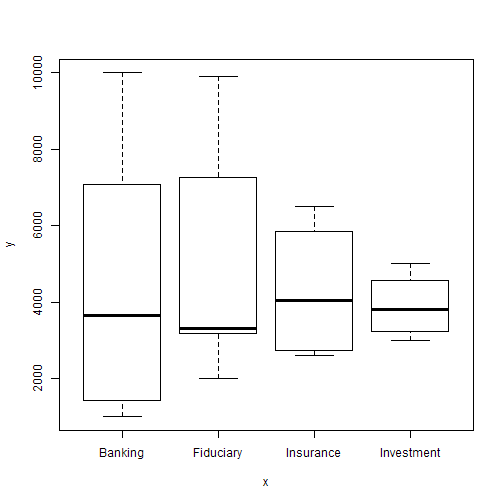
\includegraphics{r_training_data_analysis_presentation_files/figure-latex/plotting_example_1_hidden-1} \end{center}

\begin{itemize}
\tightlist
\item
  As you can see, we've specified our x and y axis, but not what type of
  plot we want
\item
  But the plot() function has guessed that we probably want a boxplot
\item
  Note: you can also force R to create a boxplot using the boxplot()
  function
\end{itemize}

\subsection{Plotting - example}\label{plotting---example-2}

\begin{itemize}
\tightlist
\item
  Next, we might want to see if there's a correlation between the meter
  reading and the temperature
\item
  Again, we can use the plot function, specify our x and y axis, and R
  will guess what the best plot is
\end{itemize}

\begin{Shaded}
\begin{Highlighting}[]
\KeywordTok{plot}\NormalTok{(}\DataTypeTok{x =}\NormalTok{ consdata}\OperatorTok{$}\NormalTok{meter_reading, }\DataTypeTok{y =}\NormalTok{ consdata}\OperatorTok{$}\NormalTok{avg_temperature_c)}
\end{Highlighting}
\end{Shaded}

\subsection{Plotting - example}\label{plotting---example-3}

\begin{center}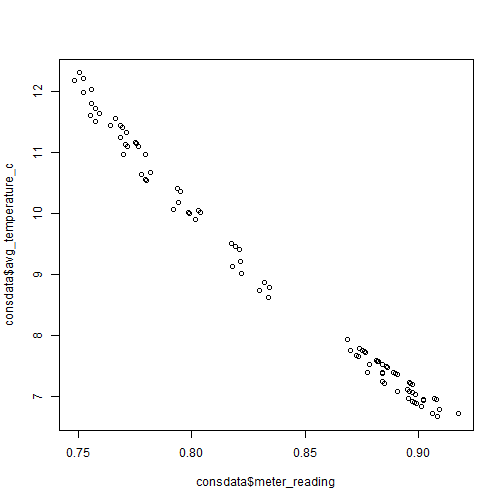
\includegraphics{r_training_data_analysis_presentation_files/figure-latex/plotting_example_2_hidden-1} \end{center}

\begin{itemize}
\tightlist
\item
  R has created a scatter plot by default, but we can change the type if
  we wish using the option ``type'' argument
\item
  See your help sheet for the different types
\end{itemize}

\subsection{Plotting - exercise}\label{plotting---exercise}

\begin{itemize}
\tightlist
\item
  Create a plot of meter readings against Settlement Periods\ldots{}
\end{itemize}

\subsection{Plotting - answer}\label{plotting---answer}

\begin{Shaded}
\begin{Highlighting}[]
\KeywordTok{plot}\NormalTok{(}\DataTypeTok{x =}\NormalTok{ consdata}\OperatorTok{$}\NormalTok{settlement_period, }\DataTypeTok{y =}\NormalTok{ consdata}\OperatorTok{$}\NormalTok{meter_reading)}
\end{Highlighting}
\end{Shaded}

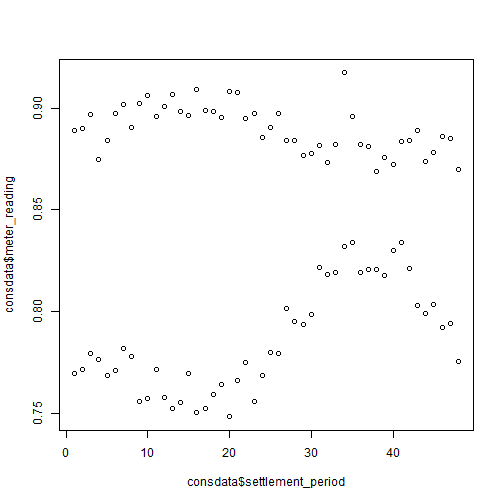
\includegraphics{r_training_data_analysis_presentation_files/figure-latex/plotting_exercise-1.pdf}

\subsection{Histograms - example}\label{histograms---example}

\begin{itemize}
\tightlist
\item
  One of the best features of the plotting system in R is how easy it is
  to make histograms
\item
  You can either use the plot() function and specify ``h'' as the type,
  or we can use the hist() function and provide one variable to produce
  a simple histogram\ldots{}
\end{itemize}

\begin{Shaded}
\begin{Highlighting}[]
\KeywordTok{hist}\NormalTok{(consdata}\OperatorTok{$}\NormalTok{meter_reading)}
\end{Highlighting}
\end{Shaded}

\subsection{Histograms - example}\label{histograms---example-1}

\begin{center}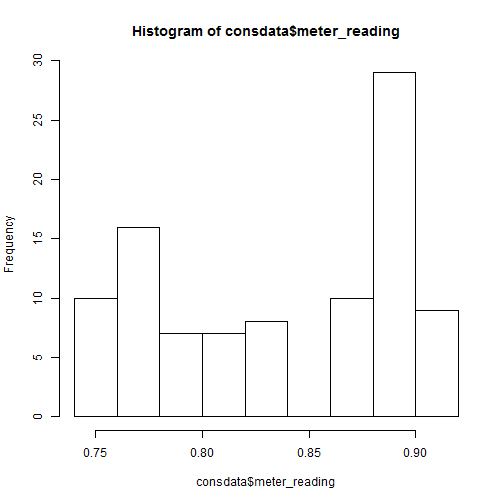
\includegraphics{r_training_data_analysis_presentation_files/figure-latex/histograms_hidden-1} \end{center}

\subsection{Customizing your graphs}\label{customizing-your-graphs}

\begin{itemize}
\tightlist
\item
  To make your graph easier to understand, you may want to\ldots{}

  \begin{itemize}
  \tightlist
  \item
    Change the title
  \item
    Change the axis labels
  \item
    Change the points
  \item
    Change the size of the bins for our histogram
  \end{itemize}
\item
  Note: These are a few of the customization options, but there are
  many, many more
\end{itemize}

\subsection{Customizing your graphs}\label{customizing-your-graphs-1}

\begin{itemize}
\tightlist
\item
  Change the title

  \begin{itemize}
  \tightlist
  \item
    To change the title, all we need to do is specify a ``main''
    parameter in our plot function\ldots{}
  \end{itemize}
\end{itemize}

\begin{Shaded}
\begin{Highlighting}[]
\KeywordTok{plot}\NormalTok{(consdata}\OperatorTok{$}\NormalTok{meter_reading, consdata}\OperatorTok{$}\NormalTok{avg_temperature_c,}
     \DataTypeTok{main =} \StringTok{"Correlation between temperature and consumption"}\NormalTok{)}
\end{Highlighting}
\end{Shaded}

\begin{itemize}
\tightlist
\item
  Change the axis labels

  \begin{itemize}
  \tightlist
  \item
    To change the labels on the axes, we use the ``xlab''/``ylab''"
    parameters\ldots{}
  \end{itemize}
\end{itemize}

\begin{Shaded}
\begin{Highlighting}[]
\KeywordTok{plot}\NormalTok{(consdata}\OperatorTok{$}\NormalTok{meter_reading, consdata}\OperatorTok{$}\NormalTok{avg_temperature_c,}
     \DataTypeTok{main =} \StringTok{"Correlation between temperature and consumption"}\NormalTok{,}
     \DataTypeTok{xlab =} \StringTok{"Meter reading (KwH)"}\NormalTok{,}
     \DataTypeTok{ylab =} \StringTok{"Temperature (degrees Celsius)"}\NormalTok{)}
\end{Highlighting}
\end{Shaded}

\subsection{Customizing your graphs}\label{customizing-your-graphs-2}

\begin{itemize}
\tightlist
\item
  Changing the graph points

  \begin{itemize}
  \tightlist
  \item
    To change the points, we use the ``pch'' paremeter, and specify a
    value between 0 and 25\ldots{}
  \end{itemize}
\end{itemize}

\begin{Shaded}
\begin{Highlighting}[]
\KeywordTok{plot}\NormalTok{(consdata}\OperatorTok{$}\NormalTok{meter_reading, consdata}\OperatorTok{$}\NormalTok{avg_temperature_c,}
     \DataTypeTok{main =} \StringTok{"Correlation between temperature and consumption"}\NormalTok{,}
     \DataTypeTok{xlab =} \StringTok{"Meter reading (KwH)"}\NormalTok{,}
     \DataTypeTok{ylab =} \StringTok{"Temperature (degress Celsius)"}\NormalTok{,}
     \DataTypeTok{pch =} \DecValTok{19}\NormalTok{)}
\end{Highlighting}
\end{Shaded}

\begin{itemize}
\tightlist
\item
  Putting those all together\ldots{}
\end{itemize}

\subsection{Customizing your graphs}\label{customizing-your-graphs-3}

\begin{center}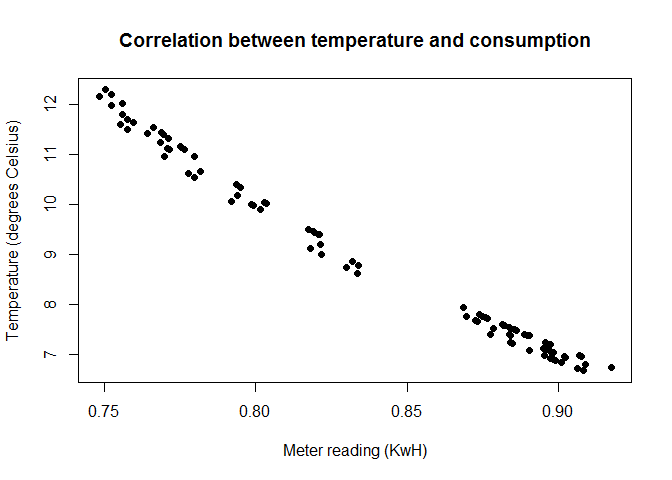
\includegraphics{r_training_data_analysis_presentation_files/figure-latex/customizing_graphs_total-1} \end{center}

\subsection{Customizing your graphs
(histograms)}\label{customizing-your-graphs-histograms}

\begin{itemize}
\tightlist
\item
  In addition to the previous customization options, for histograms, we
  can change the size of the bins

  \begin{itemize}
  \tightlist
  \item
    To do this, we specify the ``breaks'' parameter in our hist()
    function
  \item
    This splits up out our data into x number of bins of equal size
  \end{itemize}
\end{itemize}

\begin{Shaded}
\begin{Highlighting}[]
\KeywordTok{hist}\NormalTok{(consdata}\OperatorTok{$}\NormalTok{meter_reading, }\DataTypeTok{breaks =} \DecValTok{30}\NormalTok{)}
\end{Highlighting}
\end{Shaded}

\subsection{Customizing your graphs
(histograms)}\label{customizing-your-graphs-histograms-1}

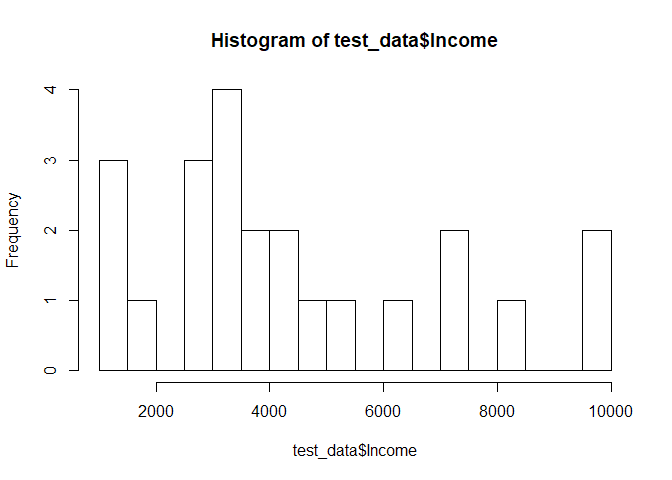
\includegraphics[width=0.5\linewidth]{r_training_data_analysis_presentation_files/figure-latex/customizing_graphs_hist_hidden-1}
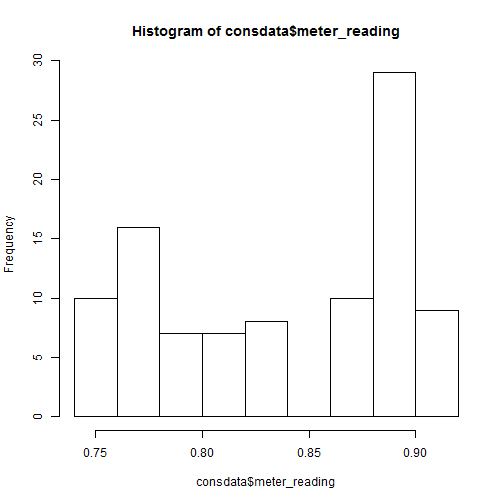
\includegraphics[width=0.5\linewidth]{r_training_data_analysis_presentation_files/figure-latex/customizing_graphs_hist_hidden-2}

\subsection{Plotting - final exercise}\label{plotting---final-exercise}

\begin{itemize}
\tightlist
\item
  Create a plot of your choice, and change the title and axis labels.
\end{itemize}

\subsection{Plotting - conclusion}\label{plotting---conclusion}

\begin{itemize}
\tightlist
\item
  In short, R has lots of in-built tools to make quick, simple graphs
  and plots
\item
  Most types of graph only require a few input parameters, but there's
  lots of customization options
\item
  In a later module, we'll look at a package called ggplot2, which we'll
  use to create more complex and professional graphics
\end{itemize}

\subsection{Conclusion}\label{conclusion}

\begin{itemize}
\tightlist
\item
  Installing packages

  \begin{itemize}
  \tightlist
  \item
    install.packages(), library()
  \end{itemize}
\item
  Loading data

  \begin{itemize}
  \tightlist
  \item
    read.csv()/read.xlsx()
  \end{itemize}
\item
  Cleaning data

  \begin{itemize}
  \tightlist
  \item
    Data type checks
  \item
    Data type conversion

    \begin{itemize}
    \tightlist
    \item
      Look out for dates and factors!
    \end{itemize}
  \end{itemize}
\item
  Plotting

  \begin{itemize}
  \tightlist
  \item
    plot()/hist()
  \end{itemize}
\item
  Customization

  \begin{itemize}
  \tightlist
  \item
    ``main'', ``xlab'', ``ylab'', ``pch'', ``breaks''
  \end{itemize}
\item
  Next time\ldots{}

  \begin{itemize}
  \tightlist
  \item
    Creating functions
  \item
    For loops
  \item
    If else statements
  \end{itemize}
\end{itemize}


\end{document}
